%\section{The $timer$ Package}
\label{app:timer-package}
Timers will be used to measure the elapsed CPU time for portions of the running code and this data will be used as input to the load balancing strategy used in the FLAME framework. The initial requirements against which the timer package was implemented are given below.

\begin{itemize}
\item Can have multiple timers running simultaneously
\item Timers can be identified individually
\item Functions to start/stop/reset a named timer
\item Function to get elapsed time from a named timer
\item Definition of a set of timers.
\item Functions to get statistics from a set of timer
\item Turn timing on/off during program execution 
\end{itemize}

We have implemented all the functionality for individual timers and a set of unit tests and an example program using the timers. Code is stored under Subversion source code control in the FLAME project on the CCPForge site. 

User documentation is supplied in \cite{TimerAPI}.

We have demonstrated the use of timers in the simple circles model by timing the work done by agents as the number of partitions over which the agents are distributed increases. The agents were not uniformly distributed in space and so, with geometric partitioning, some partitions will have more agents than others. The time taken by the agents on each node is plotted against the number of agents on the node in Figure \ref{fig:circle_timings} and we can see that there is a direct relation between the number of agents and the work done on each node. From this we can conclude that distributing the agents equally over the nodes will give a good load balance.

There is a cautionary note to be struck however. The timing data for circles has illustrated the problem identified in the overview, namely that naively giving equal numbers of agents to each node without taking into account communication can lead to worse performance. Comparing elapsed time for geometric and round robin for 5 partitions in Figure \ref{fig:timings_problems} shows that the elapsed time increased even though the work done by the agents decreased.

\begin{figure}[h]
 \centering
  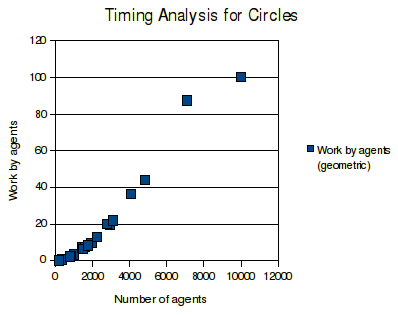
\includegraphics[scale=0.75]{circles-timings.png}
 \caption{Timings results from Circles model}
 \label{fig:circle_timings}
\end{figure}

\begin{figure}[h]
  \hspace{-10mm}
  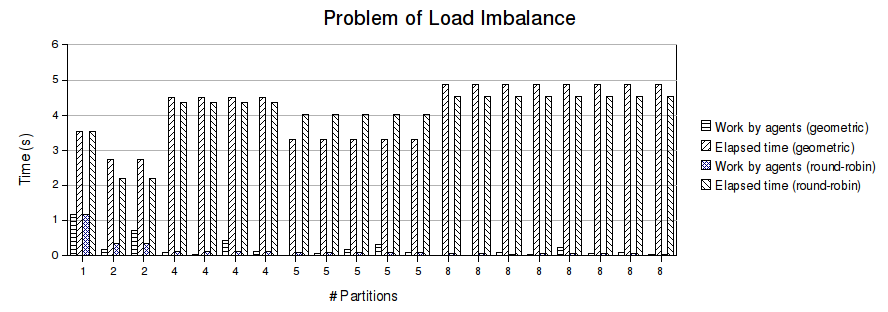
\includegraphics[scale=0.6]{timings-problems.png}
 \caption{Illustration of problems with load balancing with Circles model}
 \label{fig:timings_problems}
\end{figure}

A further example, this time from the full EURACE model, shows the top 5 elapsed times for each iteration for the first 40 iterations: see Figure \ref{fig:timing_example}.

\begin{figure}[h]
\centering
  \hspace{-10mm}
  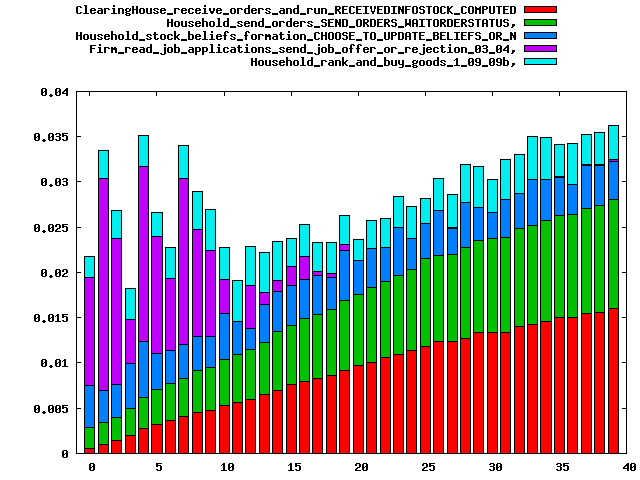
\includegraphics[scale=0.5]{timing_example.png}
 \caption{Example function timing results for EURACE Model}
 \label{fig:timing_example}
\end{figure}
